%\documentclass[a4paper,openright,12pt]{book}
%
%\usepackage[utf8]{inputenc}
%\usepackage[spanish]{babel}
%\usepackage{amsmath}
%\usepackage{fancyhdr}
%\usepackage{todonotes}
%
%% aqui definimos el encabezado de las paginas pares e impares.
%\lhead[Daniel Albendín y ángel Cantó]{Daniel Albendín y ángel Cantó}
%\chead[]{}
%\rhead[Resumen]{Resumen}
%\renewcommand{\headrulewidth}{0.5pt}
%
%% aqui definimos el pie de pagina de las paginas pares e impares.
%\lfoot[Universidad de Huelva]{Universidad de Huelva}
%\cfoot[\thepage]{\thepage}
%\rfoot[Proyecto Semandal]{Proyecto Semandal}
%\renewcommand{\footrulewidth}{0.5pt}
%
%\parskip=10pt
%
%\pagestyle{fancy} 
%
%\title{Semandal}
%\date{}
%% Este es un comentario, no será mostrado en el documento final.
%\begin{document}
%  \maketitle

\chapter*{Introducción}\addcontentsline{toc}{chapter}{Introducción}

	Actualmente en la web podemos encontrar publicada bastante información sobre municipios españoles y sus ayuntamientos, a veces el acceso a esta información es complicado debido a la diversidad en las estructuras de las páginas web de los distintos municipios ya que hay una gran variedad a la hora de realizar éstas. Existe un amplio número de frameworks que aportan una plantilla y aún así dentro de esa plantilla predefinida por el framework se puede estructurar el contenido de una forma distinta dependiendo del desarrollador. También existen páginas webs que estan encargadas a una empresa y esta usa su propia plantilla para mostrar el contenido.
	
No existe una fuente unificada de información. Si un usuario quisiera acceder a la información de distintos municipios debería consultar varias fuentes siendo él quién realice la búsqueda de los datos.
 
	Debemos dotar a la información de un significado, de una semántica, de una estructura común y adaptar la información extraida de los ayuntamientos a dicha estructura.

	La variedad de contenido en una página web al ser tan grande debemos ir paso a paso con lo que iremos analizando la información en distintas etapas.

	A parte del análisis y obtención de información, también queremos darle al usuario una forma de acceder a dicha información de una forma simplificada y estructurada, de tal forma que éste pueda consultar algo de la misma forma en cualquier ayuntamiento.


\section*{Proyecto SEMANDAL}

 \textit{Semandal} nace debido a varias necesidades como por ejemplo.
 
 \begin{enumerate}
 \item Unificación de datos en una misma fuente.
 La información de un municipio se puede encontrar en varias fuentes y el acceso a ésta depende del lugar donde esté ubicada. Si tuviésemos una fuente unificada de datos, sería mucho más sencillo el acceso a la misma.
 \item Necesidad de jerarquización y clasificación de datos.
 Los datos podemos encontrarlos, como hemos dicho antes, en distintas fuentes y con una estructura diferente en cada una de ellas. Sería bastante bueno para el posterior tratamiento de la información y el acceso, crear una ontología con los datos obtenidos.
 
 \item Acceso sencillo a dicho contenido.
 Una vez que tenemos todos estos datos, ofrecemos un sencillo acceso a dicho contenido tanto a usuarios humanos cómo máquinas. 
\end{enumerate}  

 Para la resolución de estos problema necesitamos tres partes diferenciadas en el proyecto:

\vspace{-5mm}
\begin{description}
	\item[Extracción de información] \hfill \\
		Existen bastantes datos de un ayuntamiento en su própia página web, pero tambien en documentos oficiales de los ministerios del estado o internet. \textit{Semandal} almacenará varios datos de los municipios cómo su página web, localización, deuda, población, etc \ldots  Debido a la diversidad de los datos que queremos recopilar, usaremos varias fuentes de información. Tenemos que obtener datos de fuentes muy diversas, cómo Wikipedia, Google o el INE, salvo esta última, todas tienen una forma de extracción de datos propia (Ver figura \ref{arquitecturaIntroduccion}).

\begin{figure}
\centering
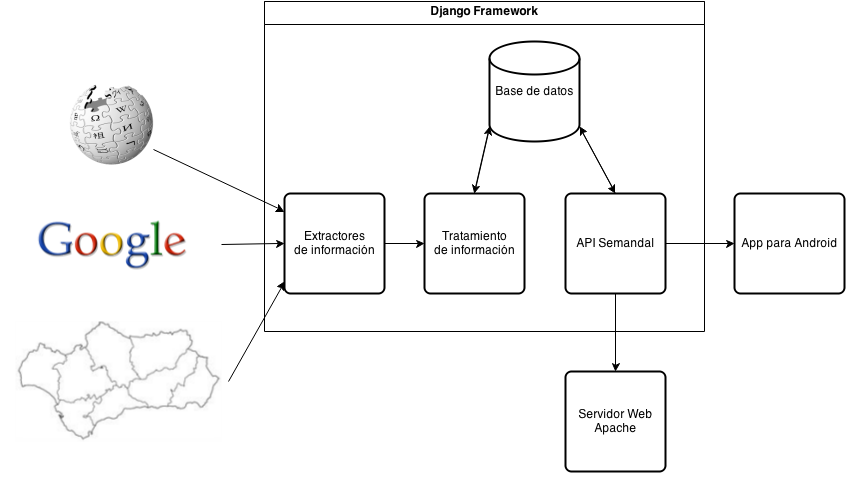
\includegraphics[scale=0.5]{./01_Resumen/ArquitecturaSemandalv5.png}
\caption{Infraestructura Semandal}
\label{arquitecturaIntroduccion}
\end{figure}




	\item [Tratamiento de la información] \hfill \\
		Aquí es donde realmente \textit{Semandal} pone su nombre en práctica y se realiza la semantización y jerarquización de datos usando técnicas de \textit{aprendizaje automático} pertenecientes al campo de la \textit{inteligencia artificial}. Le damos a la información un significado y la almacenamos de tal forma que esta pueda ser fácilmente recuperada de forma automática por un software, que es lo que usaremos para la publicación de la información.

	\item[Publicación de la información] \hfill \\
		El último pero no menos importante apartado de nuestro proyecto ya que éste será el que verá el usuario final. En este apartado es donde recopilaremos la información que hemos tratado y la mostraremos al usuario de una forma sencilla y concisa de tal forma que sea de fácil acceso tanto para usuarios humanos como para máquinas. 
		
\end{description}

Para dar soporte a las tres partes de nuestro proyecto nace una más. La infraestructura.

\begin{description}
\item[Infraestructura]
Las tres partes en las que hemos dividido el proyecto no servirían si no se pudieran sustentar en algo. Debemos crear una infraestructura que sea capaz de soportar las distintas tecnologías que vamos a utilizar en nuestro proyecto.
\end{description}

Además, a medida que se ha ido desarrollando el proyecto, se le han ido añadiendo funcionalidades de tal forma que le ha salido una parte que vimos necesaria.

\begin{description}
\item[Social]
Los usuarios podrán interaccionar entre sí además de con los distintos municipios y su contenido.
\end{description}


\section*{Objetivos}
Para cada parte del proyecto, salvo la de infraestructura ya que su único objetivo es garantizar el correcto funcionamiento de los distintos componentes del proyecto, existe un objetivo.

\begin{description}
\item[Extracción de la información]
Programar un scrapper, programa que extraiga un contenido específico, para cada fuente de información que tenemos.

\item[Tratamiento de la información] 
Crear un clasificador para transformar a la información extraída en conocimiento y la creación de una ontología.

\item[Publicación de la información]
\begin{enumerate}
\item Crear una API, conjunto de subrutinas, métodos, y procedimientos que ofrecen un servicio, para que 
\item Crear una Aplicación android (APP) que use dicha API.
\end{enumerate}

\item[Social]
 Se implementará un sistema de registro de usuarios e inicio de sesión. Así mismo, nuestra aplicación para Android tendrá un sistema donde cada usuario podrá valorar de forma positiva o negativa un comentario.
\end{description}






%\end{document}